\svnid{$Id: exporting_options.tex 80911 2026-04-14 12:40:55Z jagers $}

\chapter{Export and printing options} \label{Chp:ExportPrint}
At the end of the list of plotting options, there will always be one field that allows you to export data to a number of file formats (see \Fref{fig:4.1}).
The first section of this chapter lists what kind of file types are available under which conditions.
The second section addresses the exporting of figures for further processing.

\begin{figure}[!ht]
\center{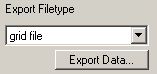
\includegraphics{Ch04/4-1.png}}
\caption{Fields for exporting the data.}
\label{fig:4.1}
\end{figure}

\section{Exporting data}
Data can be exported to a number of different file formats using the dropdown list and button shown in \Fref{fig:4.1}.
The following table lists the formats and the conditions under which the data can be exported to the indicated file format.

\begin{longtable}{|p{3.5cm}|p{3.5cm}|p{\textwidth-7cm-36pt}|}
\caption{Overview of the data export options} \\
\hline \STRUT
\textbf{Format} & \textbf{Condition} & \textbf{Comments} \\ [1ex] \hline \nopagebreak \endhead
\hline
\multicolumn{3}{r}{{\STRUT \tablename\ \thetable{} -- continued on next page}} \\
\endfoot
\endlastfoot
\STRUT
grid file & structured 2DH field, single time step & grid depends on definition of selected data field: hydrodynamic or morphologic grid \\
grid file (old format) & structured 2DH field, single time step & the old grid format with limited precision co-ordinates \\
netCDF3/netCDF4 file & unstructured 2DH field, single time step & standard 2D UGRID file, optionally compatible with D-Flow FM grid generation tools \\
Gmsh file & unstructured 2DH field, single time step & Gmsh mesh file format 2.2 or 4.1, ascii or binary \\
spline & one grid line, single time step & spline format used by \DRGFGRID\ \\
\DQUICKIN\ file & structured 2DH field & standard format for Delft3D fields \\
Delft3D-MOR field file & structured 2DH field, scalar values & obsolete file format, use \DQUICKIN\  format instead \\
SIMONA box file & structured 2DH field, scalar values & 3rd party file format, use \DQUICKIN\ format instead \\
Waqview xyz file & structured 2DH field, scalar values & 3rd party file format, use \DQUICKIN\ format instead \\
ARCview shape file & 2DH field, (not continuous shades), single time step & standard GIS format \\
GeoJSON file & 2DH, contour patches, single time step & standard GIS format \\
landboundary file & polygonal data sets & landboundary format used Delft3D \\
TEKAL file & at most 10 time steps & largely self-describing ASCII file format \\
Tecplot file & at most 10 time steps & ASCII or BINARY file format used by the visualisation program Tecplot \\
CSV file & at most 10 time steps & time-value ASCII file \\
sample file & 1 time step & x-y-value or x-y-z-value ASCII file \\
mat file & always & MATLAB binary format in three flavours (v6, v7, v7.3/hdf5) \\ [1ex] \hline
\end{longtable}

\begin{Remark}
\item Exporting large datasets to mat files may exhaust system resources.
Use \DMATLAB\ interface instead.
\item Exported data may depend on selected component and presentation type.
\end{Remark}

\section{Exporting and printing figures}\label{Sec:print_figures}
Every \QUICKPLOT\ figure contains a File menu (see \Fref{fig:4.2}).
The menu allows you to create new figures, load figures from file, close the figure, save the figure to file and, most importantly for this section, it offers you the possibility to print and export the figure.

\begin{figure}
\center{
\includegraphics{Ch04/4-2.png}}
\caption{Select the printing and exporting option from the File menu of a figure.}
\label{fig:4.2}
\end{figure}

If you select the Print/Export option from the File menu (or if you press Ctrl+P), the print/export dialog appears as shown in \Fref{fig:4.3}.
Currently, you can export your figures to the following file types: PostScript (PS), Encapsulated PostScript (EPS), TIFF, PNG and JPEG files.
On Windows PCs you have the additional option of exporting to Windows' EMF (Enhanced Meta File) format, sending the figure to the clipboard as bitmap or metafile, and you can send the figure to any of the installed Windows printers (selectable using the Options... button).

The dialog also allows you to select multiple figures to print or export.
By default only the figure from which you activated the Print/Export process is selected for printing or exporting.
If you select multiple figures, you will be asked to give a name for each figure separately.

\begin{figure}
\center{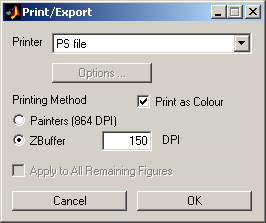
\includegraphics{Ch04/4-3.png}}
\caption{Dialog for printing and exporting figures.}
\label{fig:4.3}
\end{figure}

If you are exporting or printing to a medium that supports vector graphics (such as, PostScript files) set the printing method to painters for the best quality.
The zbuffer method will always result in a bitmap representation of the image and, therefore, it is only advantageous if the image is so complex that the painters method fails.
For the current version of \QUICKPLOT, this applies probably only to 3D plots with continuous shades.

\begin{Remark}
\item Exporting or printing a series of pictures is possible using the animation functionality as described in \Sref{Sec:AnimateResults}.
Selecting export/print as output option in the animation dialog brings up the same dialog for exporting and printing files as shown in \Fref{fig:4.3}.
\end{Remark}
